\documentclass[a4paper]{article}

%% Language and font encodings
\usepackage[english]{babel}
\usepackage[utf8x]{inputenc}
\usepackage[T1]{fontenc}

%% Sets page size and margins
\usepackage[a4paper,top=3cm,bottom=2cm,left=3cm,right=3cm,marginparwidth=1.75cm]{geometry}

%% Useful packages
\usepackage{indentfirst}
\usepackage{amsmath}
\usepackage{graphicx}
\usepackage{caption}
\usepackage{subcaption}
\usepackage{float}
\usepackage[colorinlistoftodos]{todonotes}
\usepackage[colorlinks=true, allcolors=blue]{hyperref}


\title{Calculation of hydrogen-air mixtures detonation parameters using EDL Shock \& Detonation Toolbox}
\author{Łukasz Osiński}

\begin{document}
\maketitle

\begin{abstract}
The aim of this report was to calculate detonation cell size using ZND in SD Toolbox for Cantera 2.1 and detonation parameters as a function of variable initial temperature.
\end{abstract}

\section{Detonation theory}
The one-dimensional detonation model developed independently by Zeldovich, von Neumann and Doring (called ZND for short) during World War II assumes that a detonation wave consist of a planar shock wave, which raises the density above the ignition value,  followed by a reaction zone in which reaction proceeds. Experiments data confirms the model only qualitatively, because one-dimensional detonation waves are unstable.\cite{G_Summary}. The model is simple to implement computationally.

It was proposed by Schelkin and Torshin in 1963 that detonation cell size can be related to reaction zone length $\Delta$ calculated using the ZND model \cite{Ciccarelli} via simple equation: $\lambda=A*\Delta$ (where $\Delta=(V_{CJ}-u)*t_{ind}$,  $V_{CJ}$ is C-J speed and $u$ is the particle velocity behind the shock wave).
However experiments prove that constant $A$ ratio cannot be accurate. Instead, it was proposed that $A$ should be a function of initial conditions. Shepherd in 1986 proposed, that $A = f(\Phi)$, because large variations of this parameter with equivalence ratio are observed \cite{Remy}.

\section{Part 1 - ZND calculations}
\subsection{Model}

The computation was made in Matlab for hydrogen  – air mixture (file: $ZNDCJ.m$) with equivalence ratio ranging from 0.4875 to 3.57 in points taken from experiments performed by Guirao et al.\cite{Guirao}. (Not all points were tested). The initial conditions were: pressure = 101300 Pa , temperature= 293 K.Then knowing that cell size is proportional to reaction zone lenght , and that the constant of proportionality $A$ was determined to be equal to 51 by Ciccarelili et al.\cite{Ciccarelli}. Cell size can be calculated based on induction zone length, which is a output data for ZND program in SD Toolbox. 
\subsection{Results}

Figure \ref{fig:ind_t_and_l} shows the output data, and Figure \ref{fig:ZND_cell_size} compares the acquired cell size with experimental data taken from work of Guirao et al.\cite{Guirao} \cite{DetDat}. The error was ranging from $7.35\%$ to $68.88\%$ with mean error for all points of $46\%$.

\begin{figure}[h!]
\centering
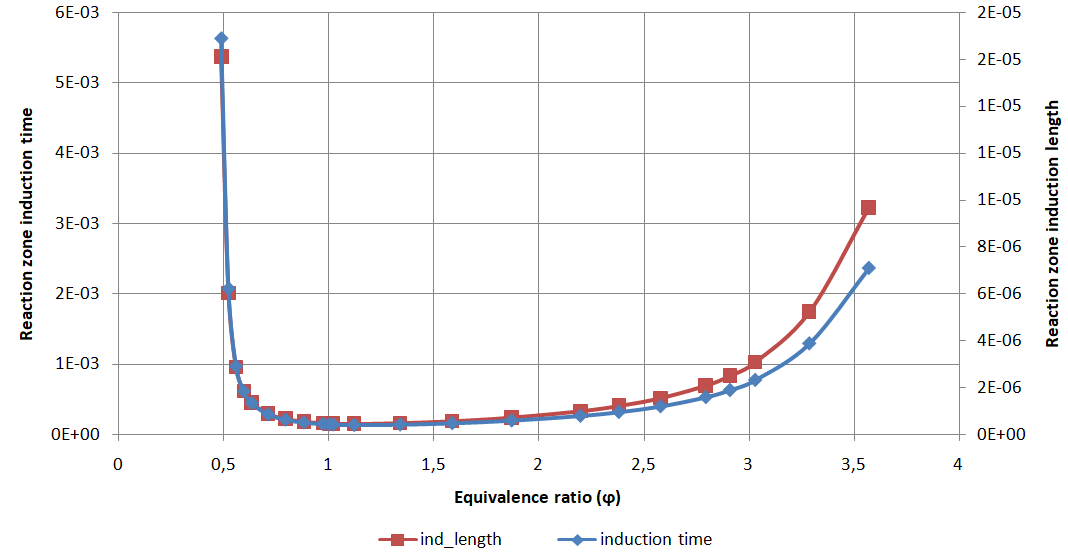
\includegraphics[width=1\textwidth]{1_ind_time_AND_ind_zone_length_against_eq_ratio.PNG}
\caption{\label{fig:ind_t_and_l}Induction time and ind. length as a function of equivalence ratio}
\end{figure}

\begin{figure}[H]
\centering
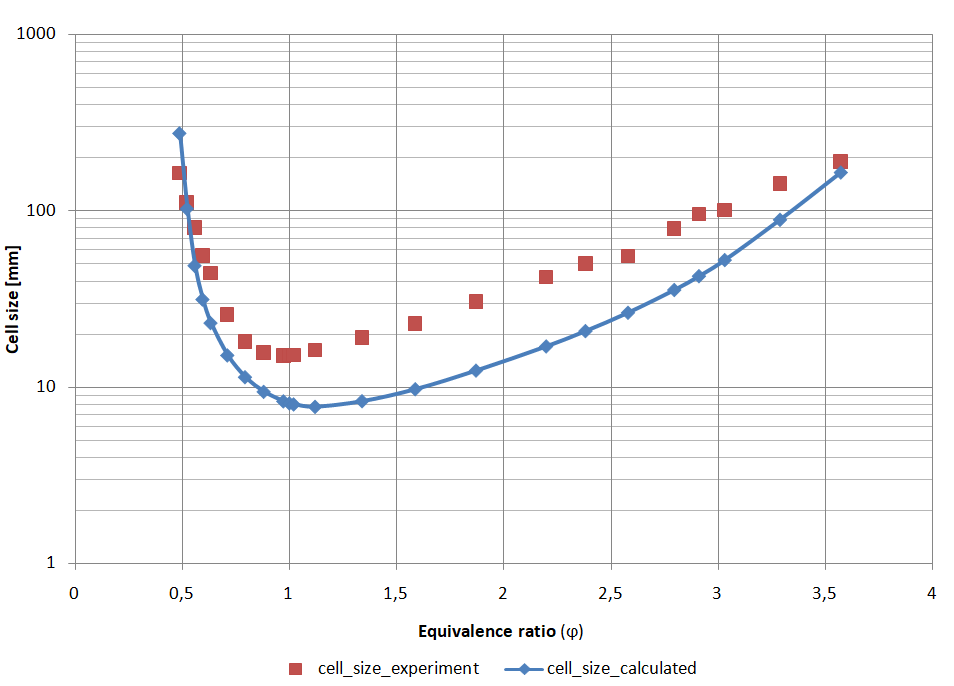
\includegraphics[width=1\textwidth]{1_cell_size_against_phi.PNG}
\caption{\label{fig:ZND_cell_size}Calculated detonation cell size as a function of equivalence ratio}
\end{figure}

Plotting the A factor, which was calculated basing on actual cell size from experiment (\cite{Guirao}) and computed induction lengths as a function of equivalence ratio yields Figure \ref{fig:A_exp}. As can be observed the A factor varies to the greatest extent below $\Phi = 1.12$ and above $\Phi = 2.38$. Between those points the average A factor is equal to 119.1, which is two times higher than the value obtained in experiment by Ciccarelili et al.\cite{Ciccarelli}.

\begin{figure}[H]
\centering
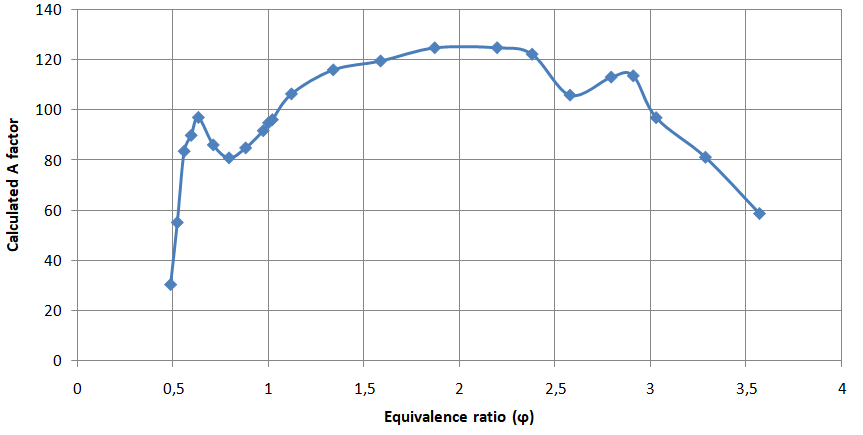
\includegraphics[width=1\textwidth]{1_A_calculated.PNG}
\caption{\label{fig:A_exp}Calculated factor of proportionality $A$ as a function of equivalence ratio}
\end{figure}

\section{Part 2 - Detonation parameters as a function of initial temperature}
\subsection{Model}

The second task was to determine detonation parameters with variable initial temperature. This was done using SD Toolbox in Matlab, using modified example code (file: $Temperature\_Series.m$) The temperature was ranging from $300 K$ to $1000  K$ with a step of $50 K$. Pressure was set to $100000 Pa$. The equivalence ratio was constant and equal to 1.
\subsection{Results}

Results are shown on Figures \ref{fig:part2_1} to \ref{fig:part2_5}.

\begin{figure}[H]
\centering
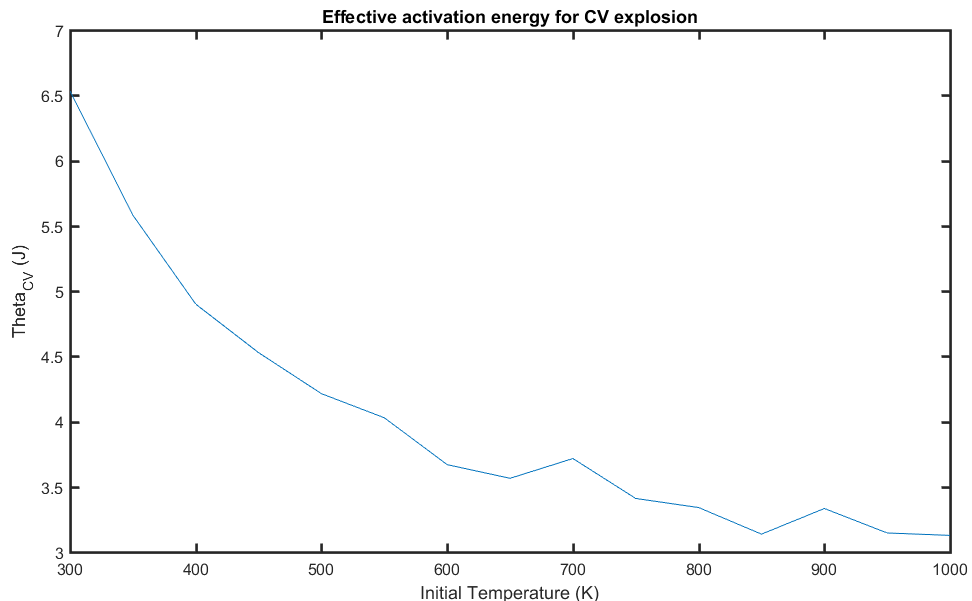
\includegraphics[width=0.75\textwidth]{2_eff_act_energy_CVexpl.png}
\caption{\label{fig:part2_1}Calculated effective activation energy for CV explosion as a function of temperature}
\end{figure}

\begin{figure}[H]
\centering
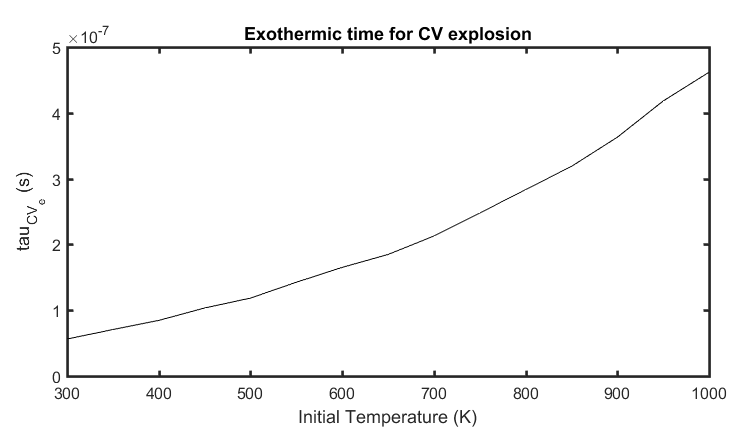
\includegraphics[width=0.75\textwidth]{2_exothermic_time.png}
\caption{\label{fig:part2_2}Calculated exothermic time as a function of temperature}
\end{figure}

\begin{figure}[H]
\centering
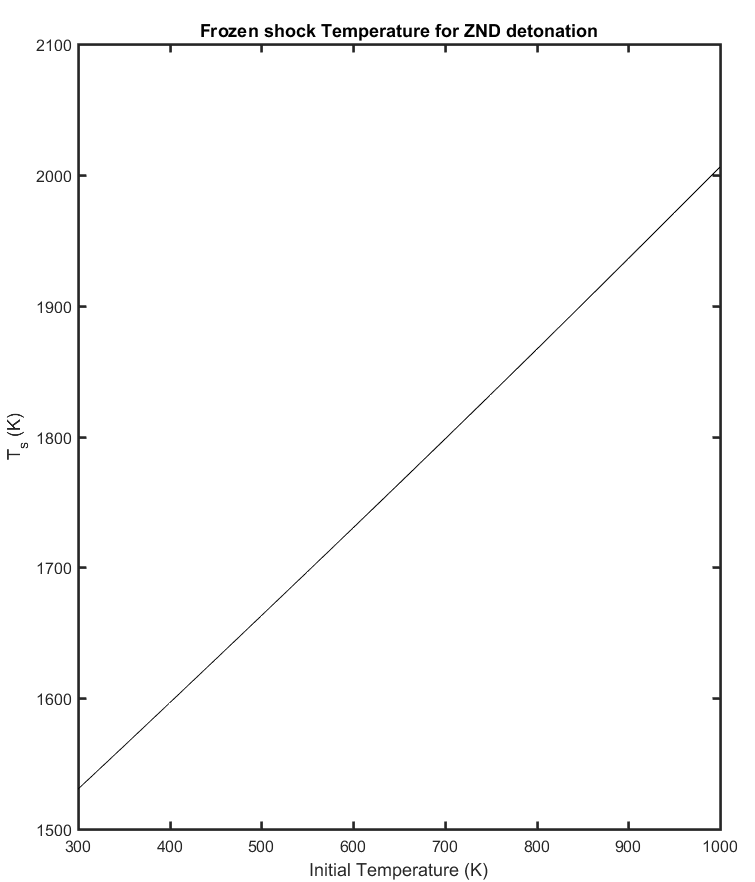
\includegraphics[width=0.75\textwidth]{2_frozen_schock_temperature.png}
\caption{\label{fig:part2_3}Calculated frozen shock temperature as a function of temperature}
\end{figure}

\begin{figure}[H]
\centering
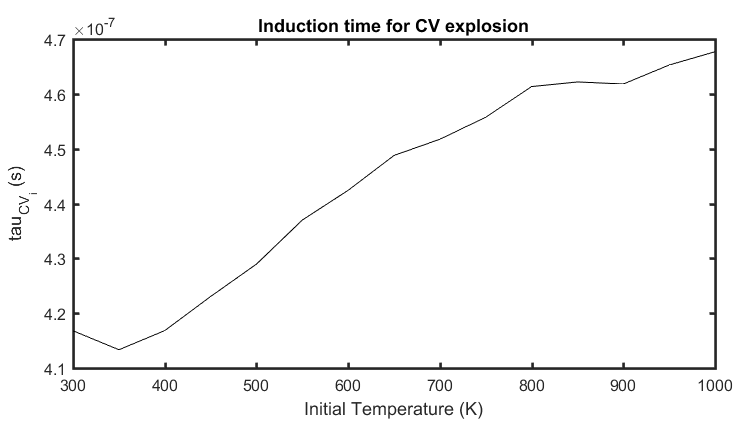
\includegraphics[width=0.75\textwidth]{2_ind_time_CV_expl.png}
\caption{\label{fig:part2_4}Calculated as a function of temperature}
\end{figure}

\begin{figure}[H]
\centering
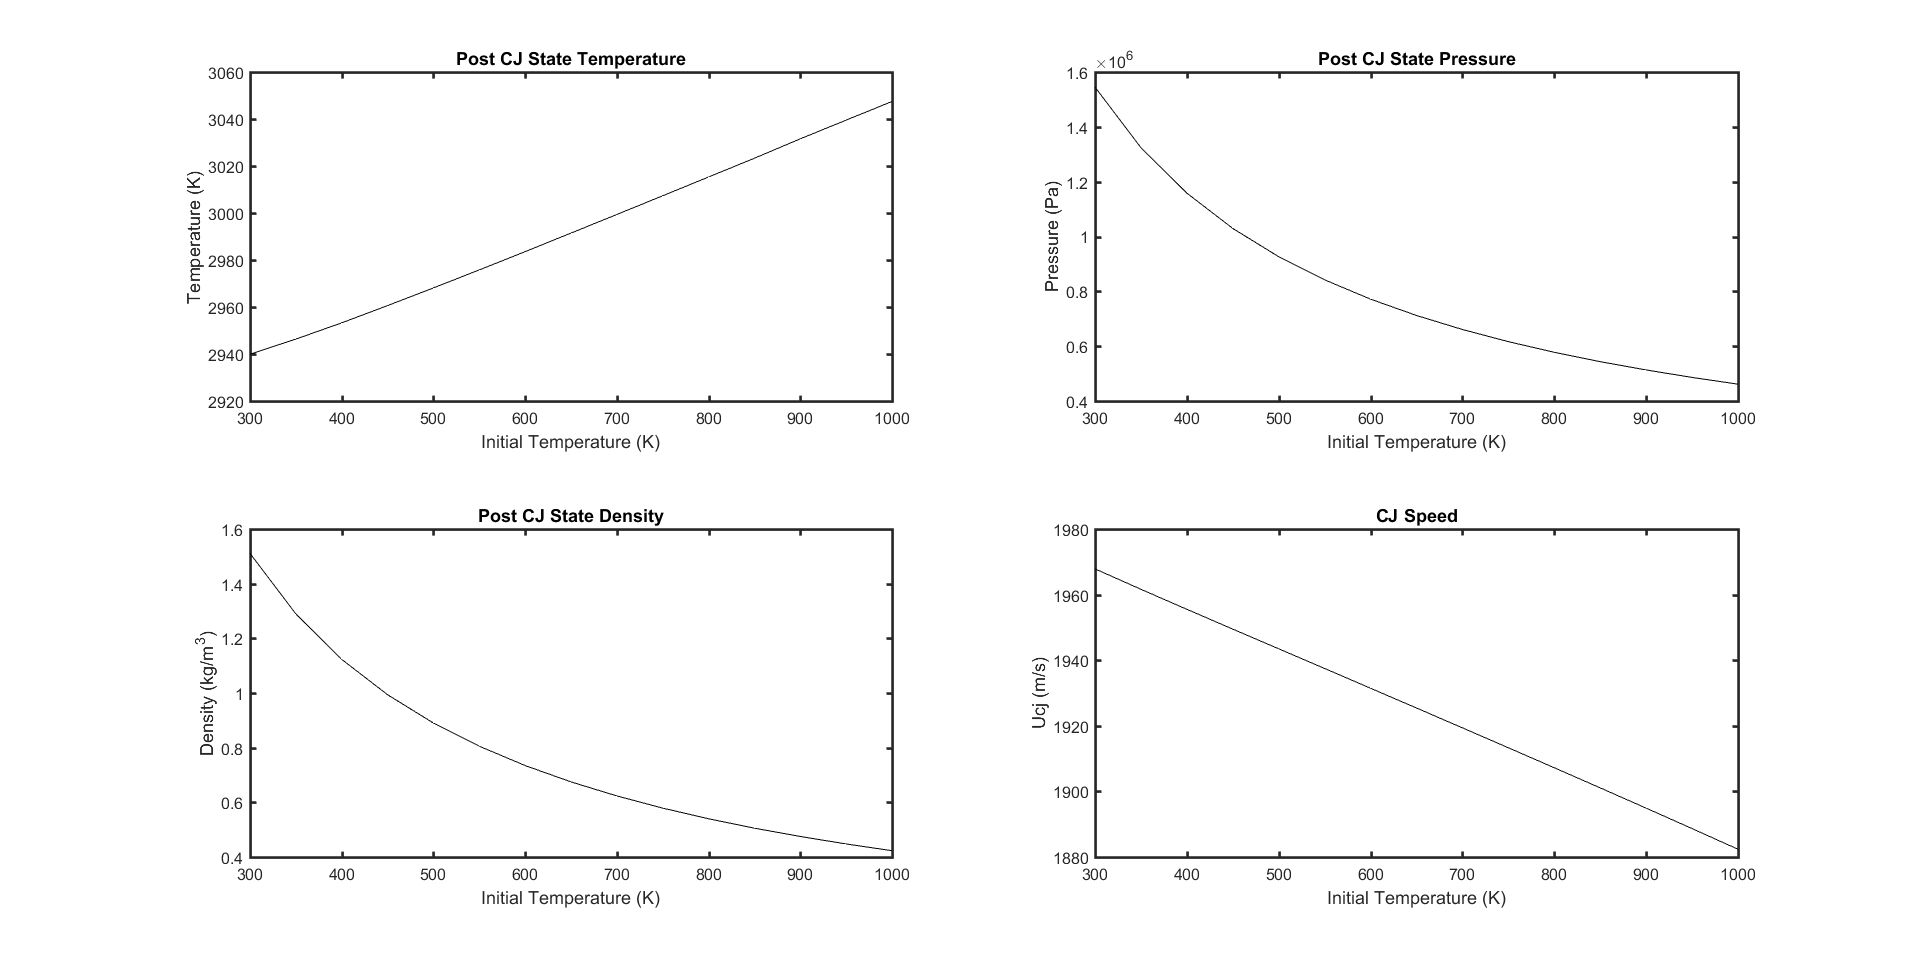
\includegraphics[width=1\textwidth]{2_post_CJ.png}
\caption{\label{fig:part2_5}Calculated induction time as a function of temperature}
\end{figure}


\section{Conclusions}

Calculations from the first part of the report prove that using constant $A$ factor, independent from $\Phi$  will not accurately predict real cell sizes.

In the second part of the report we can see that effective activation energy is dropping non-linearly with rising temperature and exothermic time is rising non-linearly.
Frozen shock Temperature is linearly related to initial temperature by equation $T_S=0.679*T_1+1324$.
Induction time for CV explosion and post CJ state temperature rise with the rise of initial temperature. Rise of post CJ state temperature is linear and governed by equation: $T_2=0.155*T_1+2891$.
Post CJ pressure and density declines with the rise of initial temperature. The drop of CJ speed with rising temperature is linear and can be described as $V_{CJ}=-0.121*T_1+2004$.

\bibliographystyle{unsrt}
\bibliography{ref}

\end{document}